% -*- coding: utf-8 -*-
% \documentclass[journal]{IEEEtran}
\documentclass[titlepage, twocolumn, a4paper, 10pt]{article}
\usepackage{parskip}
\usepackage[english]{babel}
\usepackage[utf8]{inputenc}
\usepackage{verbatim}
\usepackage{fancyhdr}
\usepackage{graphicx}
\usepackage{url}
\usepackage{varioref}

%%%%%%%%%%%%%%%%
% Column spacing
% \setlength{\columnsep}{7mm}
\renewcommand{\sfdefault}{phv}
\renewcommand{\rmdefault}{ptm}
\renewcommand{\ttdefault}{pcr}

\hyphenpenalty=750
% If we didn't adjust the interword spacing, 2200 might be better.
% The TeX default is 1000
\hbadness=1350
% IEEE does not use extra spacing after punctuation
\frenchspacing

% V1.7 increase this a tad to discourage equation breaks
\binoppenalty=1000 % default 700
\relpenalty=800     % default 500


% margin note stuff
\marginparsep      10pt
\marginparwidth    20pt
\marginparpush     25pt


% if things get too close, go ahead and let them touch
\lineskip            0pt
\normallineskip      0pt
\lineskiplimit       0pt
\normallineskiplimit 0pt

\topmargin    -49.0pt
\headheight   12pt
\headsep      0.25in

\textheight       58pc  % 9.63in, 696pt
\columnsep         1pc
\textwidth        42pc   % 2 x 21pc + 1pc = 43pc

% the default side margins are equal
\oddsidemargin        0.680in
\evensidemargin       0.680in
% compensate for LaTeX's 1in offset
\addtolength{\oddsidemargin}{-1in}
\addtolength{\evensidemargin}{-1in}
\topmargin        -0.25in
% we retain the reserved, but unused space for headers
\addtolength{\topmargin}{-\headheight}
\addtolength{\topmargin}{-\headsep}

%%%%%%%%%%%%%%%%


\usepackage[pdfborder={0 0 0 0}]{hyperref}

% Include pdf with multiple pages ex \includepdf[pages=-, nup=2x2]{filename.pdf}
\usepackage[final]{pdfpages}

% Place figures where they should be use [H]
\usepackage{float}

% Float for text
\floatstyle{ruled}
\newfloat{code}{!htb}{lop}
\floatname{code}{CodeSnippet}

% vars
\def\title{Umume}
\def\preTitle{A RESTful service}
\def\kurs{Service-Oriented Architectures, HT-09}


\def\namn{Anton Johansson}
\def\mail{dit06ajn@cs.umu.se}

\def\namnTva{Jonny Strömberg}
\def\mailTva{dit06jsg@cs.umu.se}


\def\pathtocode{\url{dit06ajn~/edu/soa/umume}}
\def\handledareEtt{P-O Östberg, p-o+soa@cs.umu.se}

\def\inst{Computer Science}
\def\dokumentTyp{Report}

\begin{document}
\begin{titlepage}
  \thispagestyle{empty}
  \begin{small}
    \begin{tabular}{@{}p{\textwidth}@{}}
      UMEÅ UNIVERSITY \hfill \today \\
      Department of \inst \\
      \dokumentTyp \\
    \end{tabular}
  \end{small}
  \vspace{10mm}
  \begin{center}
    \LARGE{\preTitle} \\
    \huge{\textbf{\kurs}} \\
    \vspace{10mm}
    \LARGE{\title} \\
    \vspace{15mm}
    \begin{large}
      \namn, \mail \\
      \namnTva, \mailTva\\
      % Code-path: \texttt{\pathtocode}\\
      \vspace{10mm}
    \end{large}
    \vfill
    \large{\textbf{Supervisors}}\\
    \mbox{\large{\handledareEtt}}\\
  \end{center}
\end{titlepage}

\newpage
\mbox{}
\vspace{70mm}
\begin{center}
  % Dedication goes here
\end{center}
\thispagestyle{empty}
\newpage

\pagestyle{fancy}
\rhead{\today}
\lhead{\footnotesize{\namn, \mail\\\namnTva, \mailTva}}
\chead{}
\lfoot{}
\cfoot{}
\rfoot{}

\cleardoublepage
\newpage
\onecolumn
\tableofcontents
\twocolumn
\cleardoublepage

\fancyfoot[LE,RO]{\thepage}
\pagenumbering{arabic}

\section{Introduction}\label{sec:intro}
% Beskriv med egna ord vad uppgiften gick ut på. Är det någonting som
% varit oklart och ni gjort egna tolkningar så beskriv dessa.
This report describes the work done designing and implementing a RESTful web service providing information about employees and students at Umeå university. For this web service a client web site is done to highlight possible uses of the web service.

The main idea with the web service is to combine information from the existing information about every employee/student with a possibility for persons to add information about themselves. This information can for example be a brief description, visiting location and usernames for other web services such as Twitter\footnote{\url{http://twitter.com/}} to enable mashup implementations.

The web service will hereby be called \textit{Umume-rest}, a combination of \textit{Umu} as in Umeå university and {me} because it provides a service for students and employees. The client web site is called \textit{Umume-website}. All students and employees at Umeå university are potential users of our service, they will herby be refereed to as users.

These implementations are done with the programming language
\textit{Java}\footnote{\url{http://java.sun.com/}} and uses the framework \textit{Spring Framework}\footnote{\url{http://www.springframework.org/}} for the web site, and \textit{Jersey}\footnote{\url{https://jersey.dev.java.net/}} for the RESTful Web service.

The original project specification for this work is shown in Appendix \ref{app:ps}.

\section{Problem analysis}\label{sec:problem-analysis}
% As this project emphasizes analysis and investigation of a loosely
% specified problem, include any assumptions you made during the
% analysis phase in your report. Also discuss problems encountered and
% alternative solutions considered in the analysis. The report should
% also discuss to what extent the requirement list is fulfilled, as
% well as to which extent you could adhere to the the project plan.
Since the \textit{Umume-rest} is created to enable third party developers to access information and create their own web service, it was decided to make the web service RESTful instead of using the SOAP protocol. This decision was made because in a RESTful web service every resource have a unique identifier easily accessible with a simple HTTP GET method call. For example the information about a person could be fetched by pointing a web browser to \url{http://example.com/users/aonjon04}. This for example enables the development of simple AJAX Javascript clients that use our service, this is demonstrated and described in Section \ref{sec:TODO}.

The web service \textit{Umume-rest} builds mainly on two existing services provided by Umeå university, a Lightweight Directory Access Protocol directory service (LDAP) and a Central Authentication Service (CAS).

\subsection{LDAP}\label{sec:ldap}
All preexisting informations about users is fetched from an LDAP directory service provided by the university at \url{ldap://ldap.umu.se}. This directory service contains information about every student and employee. Every user is uniquely identified by a 8 character string such as "aonjon04". With every unique user comes extra information such as faculty membership, email addresses, phone numbers and so on.

An initial idea was to use address information about every user and map this information to a longitude and latitude to plot the users positions an a map, for example by using Google Maps API\footnote{\url{http://code.google.com/apis/maps/}}. This idea was however discarded since the structure of location information from LDAP was inconsistent between different users and faculties.

The most important service provided by LDAP used by \textit{Umume-rest} is the possibility to search for first- and surnames to retrieve their unique CAS-username. This username is used to authenticate users, see the following section.

\subsection{Central Authentication Serive}\label{sec:cas}
Every employee and student at Umeå university can get a CAS-user and password by physically visiting a reception and identifying themselves. This CAS-user enables access to different services around campus, for example accessing the wireless network, scientific articles and checking results from finished courses. More information about CAS can be found at \url{http://www.it.umu.se/vara-tjanster/centralt-anvandarnamn/cas/} (in Swedish).

The CAS used by \textit{Umume-rest} is located at \url{https://cas.umu.se/} and is used by \textit{Umume-rest} to authenticate requests to add or change information about your own user. This means that no extra username or password is required for users or \textit{Umume-rest} and users can only edit their own information.

% TODO: Discuss single point of failure?

\section{Compilation and deployment}\label{sec:compile}

All files needed to use set up the web service are located at:\\
\texttt{\pathtocode}/umume-rest and the files for the web site are at:\\
\texttt{\pathtocode}/umume-website


\subsection{Servlet container}\label{sec:usage-servlet-container}
This project has been developed with \textit{Apache Tomcat 6.0.20}\footnote{http://tomcat.apache.org/} as servlet container but any Java servlet 
container should do.

\subsection{Web service - umume-rest}
This section explains how to understand, compile and use
\textit{umume-rest}.
This catalog contains the following sub directories:
\begin{itemize}
\item \verb!src! contains the source code.
\item \verb!src/main/resources/! contains the SQLite database and 
the configuration
  files for standard behaviour of the compiled system, see section
  \ref{sec:configuration}. 
\item \verb!target! will, after a successful compilation,
  contain all the compiled sources as well as configuration files used
  by this web service.
\item \verb!lib! contains all requires third-party libraries
  needed by the \textit{Umume web service}.
\item \verb!conf! contains the build-properties file and the jar-file for Ivy.
\end{itemize}

And these are the files in the catalog:
\begin{itemize}
\item \verb!build.xml! contains settings for building this web service.
\item \verb!ivy.xml! contains all Ivy dependencies. 
\item \verb!ivysettings.xml! contains the Ivy settings. 
\end{itemize}

\subsubsection{Compilation}\label{sec:compilation-rest}
The following commands will require the software tool \textit{Apache
  Ant}\footnote{http://ant.apache.org/}. More details about what
happens using \textit{ant} in this project is found in the file
\textit{build.xml}\footnote{http://ant.apache.org/manual/using.html}.

To deploy \textit{umume-rest} issue the following command:\\
\begin{footnotesize}
  \verb!salt:./umume-rest> ant deploy!
\end{footnotesize}\\
This will create a directory \verb!target! if it does not already exists
and compile/move source-code and configuration files to that
directory. Then a war file is generated and moved to the servlet 
container (remember to configure the build properties in 
\verb!conf/build.properties!)

The root-directory for class-files when using \textit{umume-rest} is
compiled to \textit{target/classes/}, while the root-directory for
test-code is compile to \textit{target/test-classes/}.

To create portable \textit{war}-file of the compiled sources issue the
following command:\\
\begin{footnotesize}
  \verb!salt:./umume-rest> ant war!
\end{footnotesize}\\
This will create \textit{umume-rest.war} which can be deployed within
any Java servlet container.


\subsection{Web site - umume-website}

This catalog contains the following relevant sub directories:
\begin{itemize}
\item \verb!src! contains the source code.
\item \verb!war/WEB-INF/jsp/! contains all .jsp-files used for the web site design.
\item \verb!war/WEB-INF/classes/! will, after a successful compilation,
  contain all the compiled source files.
\item \verb!war/WEB-INF/lib! contains all requires third-party libraries
  needed by \textit{umume-website}.
\item \verb!war/WEB-INF/tld/! contains Spring specific librarys.
\item \verb!war/css/! contains the css stylesheet.
\item \verb!war/images/! contains all images displayed on the web site.
\item \verb!war/js/! contains all javascript-files.
\end{itemize}

And these are the interesting files in \textit{umume-website}:
\begin{itemize}
\item \verb!build.xml! contains settings for building this web service.
\item \verb!ibuild.properties! contains the build properties. 
\item \verb!iwar/WEB-INF/umume-servlet.xml! contains definitions of
all views and beans used in \textit{umume-website}.  
\item \verb!iwar/WEB-INF/web.xml! contains definitions of filers, sevlets and
taglibs used in \textit{umume-website}. 
\item \verb!iwar/WEB-INF/urlrewrite.xml! contains rules for URL rewriting. 
\end{itemize}

\subsubsection{Compilation}\label{sec:compilation-website}
The following commands will require the software tool \textit{Apache
  Ant}\footnote{http://ant.apache.org/}. More details about what
happens using \textit{ant} in this project is found in the file
\textit{build.xml}\footnote{http://ant.apache.org/manual/using.html}.

To deploy \textit{umume-website} issue the following command:\\
\begin{footnotesize}
  \verb!salt:./umume-website> ant deploy!
\end{footnotesize}\\
This will create a directory \verb!war/WEB-INF/classes! if it does not already exists
and compile/move source-code and configuration files to that
directory. Then the catalog is copied the the pre-defined servlet container
(\verb!conf/build.properties!).

To create portable \textit{war}-file of the compiled sources issue the
following command:\\
\begin{footnotesize}
  \verb!salt:./umume-rest> ant deploywar!
\end{footnotesize}\\
This will create \textit{umume.war} which can be deployed within
any Java Servlet container.



\section{Usage}\label{sec:usage}
% Förklara var programmet och källkoden ligger samt hur man kompilerar,
% startar och använder det. Förklara även översiktligt vad som händer
% när man använder de olika kommandona. Det räcker alltså inte att
% skriva "man skriver 'ant' för att kompilera", utan det måste även ingå
% en liten förklaring om vad som egentligen händer när man kör ant och
% varför det fungerar. Använd Internet eller litteratur för att själva
% ta reda på den information ni tycker känns relevant, dels för
% rapportens skull och dels för er egen. Kom ihåg att skriva tydliga
% (vetenskapliga) referenser!

This description explains how to communicate with the web sercive and
how to navigate on the web site.

\subsection{Web service - umume-rest}
There are two different resources in the service. Both allows GET requests and
and one of them also allows
authorised users to add or change information with PUT.
\begin{itemize}
    \item GET \verb!/users/{uid}! returns information about a user in either
    \textit{application/xml} or \textit{application/json} depending on which the user 
    requested. 
    \item PUT \verb!/users/{uid}?ticket={CAS-ticket}&service={service-url}! updates information about the specified user if the request contains a CAS-ticket and a service-URL that validates. The
    format of the request is \textit{application/xml}. For more information se \ref{code:put-request}
    \item GET \verb!/search/{searchString}! returns a list of users matching the provided 
    search string in either
    \textit{application/xml}, \textit{application/json} or \textit{application/javascript}
     depending on which the user requested.
\end{itemize}

\begin{code}
  \begin{footnotesize}
\begin{verbatim}
<person ref="http://mega.cs.umu.se:8080/umume-rest/users/jost0038">
    <description>My own description</description>
    <latitude>0.0</latitude>
    <longitude>0.0</longitude>
    <twitterName>MyTwitterName</twitterName>
</person>
\end{verbatim}
  \end{footnotesize}
  \caption{PUT request example}\label{code:put-request}
\end{code}

\subsection{WADL}

The methods available for clients of \textit{Umume-rest} is available in a  Web Application Description Language (WADL\footnote{\url{http://www.w3.org/Submission/wadl/}} file \texttt{application.wadl} located at the base of all the resources. See the complete WADL for \textit{Umume-rest} in Appendix \ref{app:wadl}.

\subsection{Web site - umume-website}

The following images describes how to navigate through 
the \textit{umume-website}.

\begin{figure}[!thb]
  \centering
  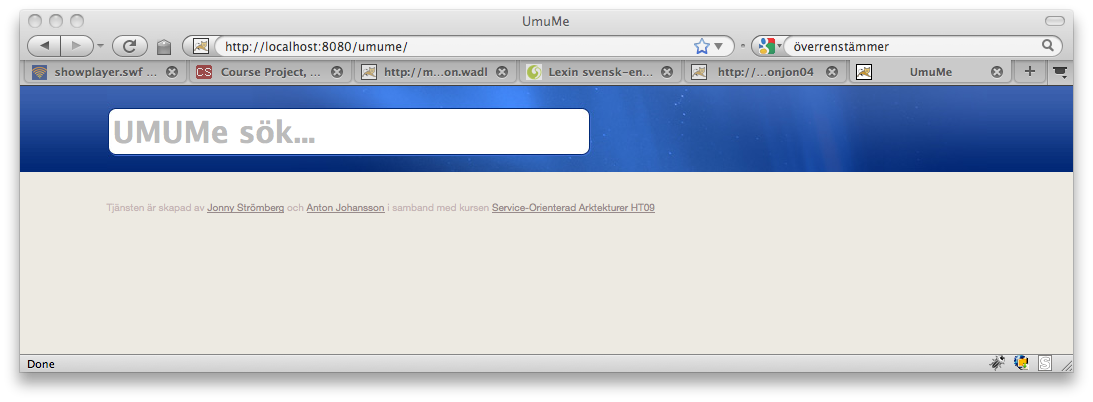
\includegraphics[width=3.3in]{images/pic1.png}
  \caption{Start page.}
  \label{fig:images/startpage}
\end{figure}

\begin{figure}[!thb]
  \centering
  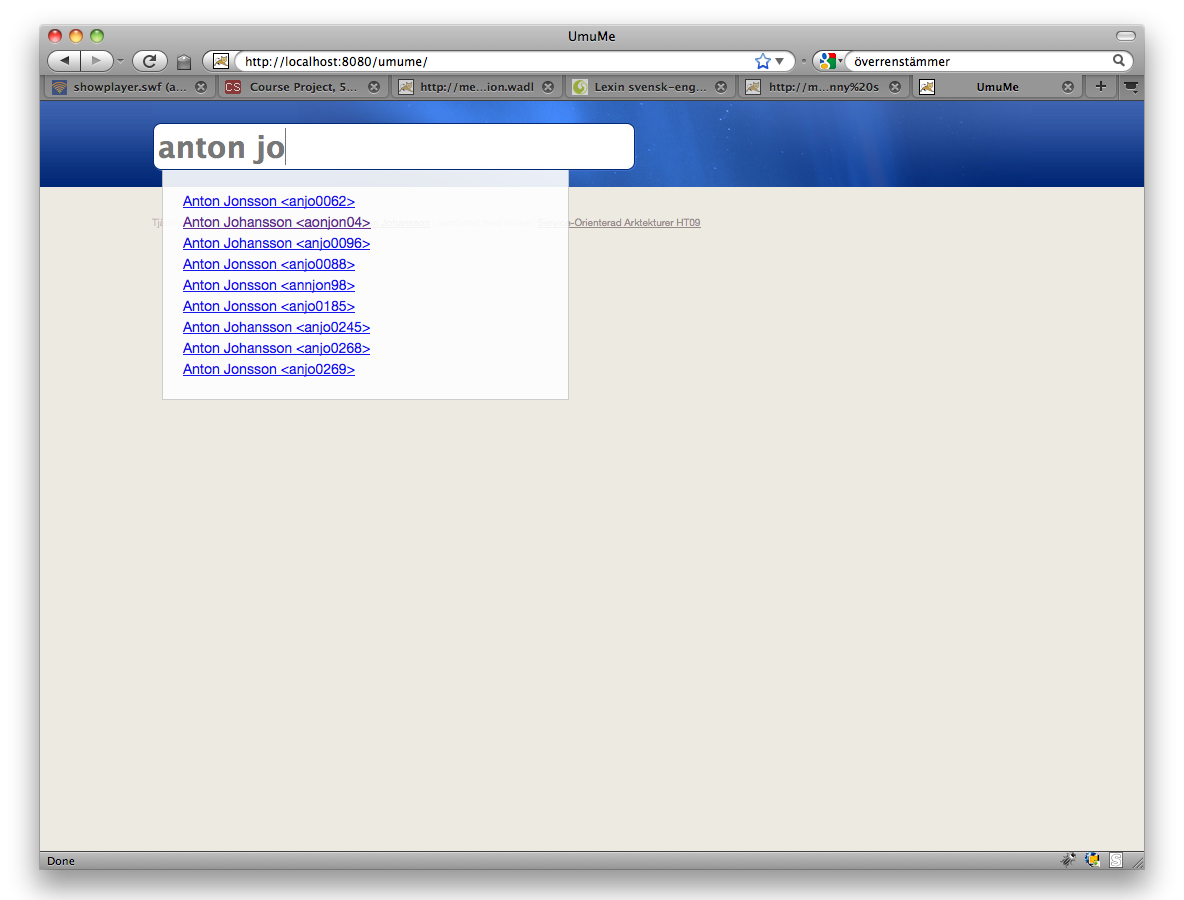
\includegraphics[width=3.3in]{images/pic2.png}
  \caption{Search for persons.}
  \label{fig:images/search}
\end{figure}

\begin{figure}[!thb]
  \centering
  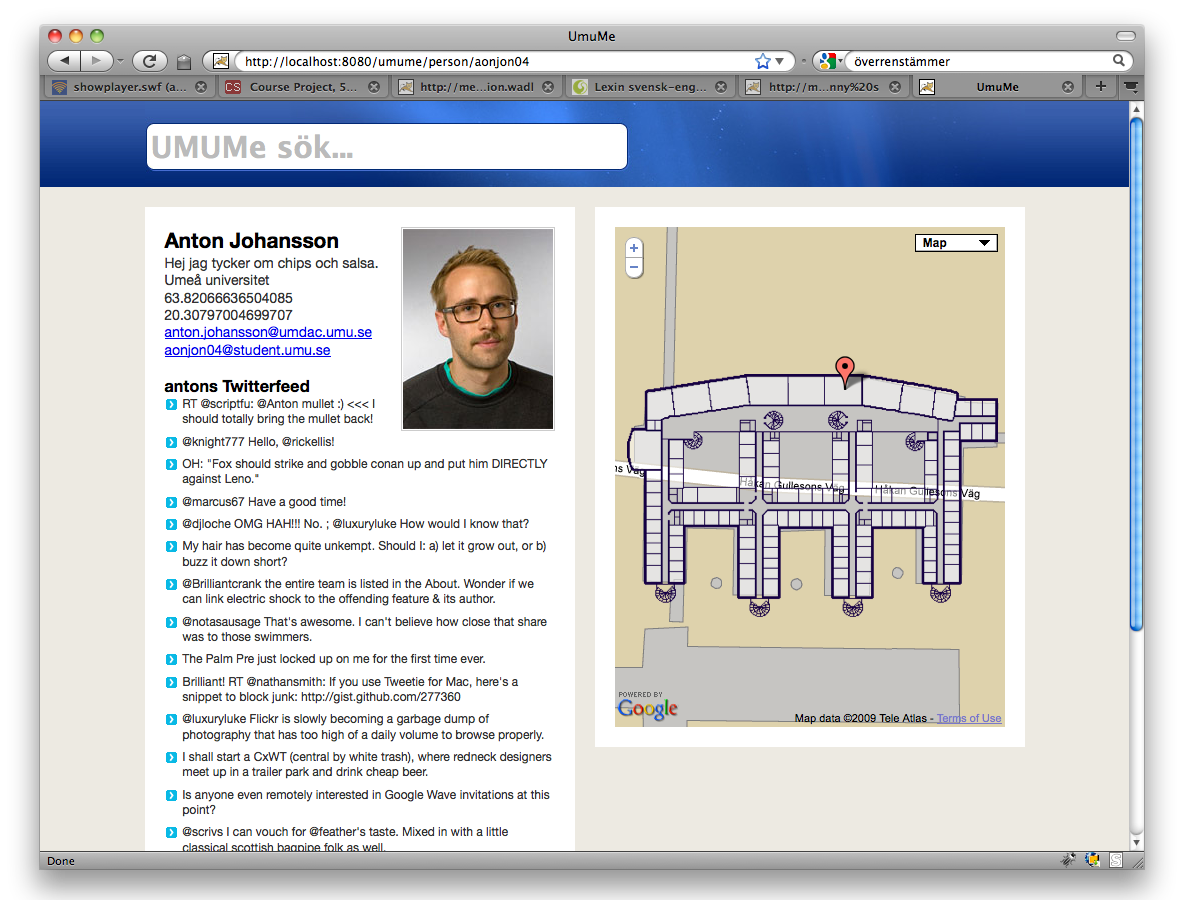
\includegraphics[width=3.3in]{images/pic3.png}
  \caption{User profile, eventually with Twitter-feed and position at Google Maps.}
  \label{fig:images/person}
\end{figure}

\begin{figure}[!thb]
  \centering
  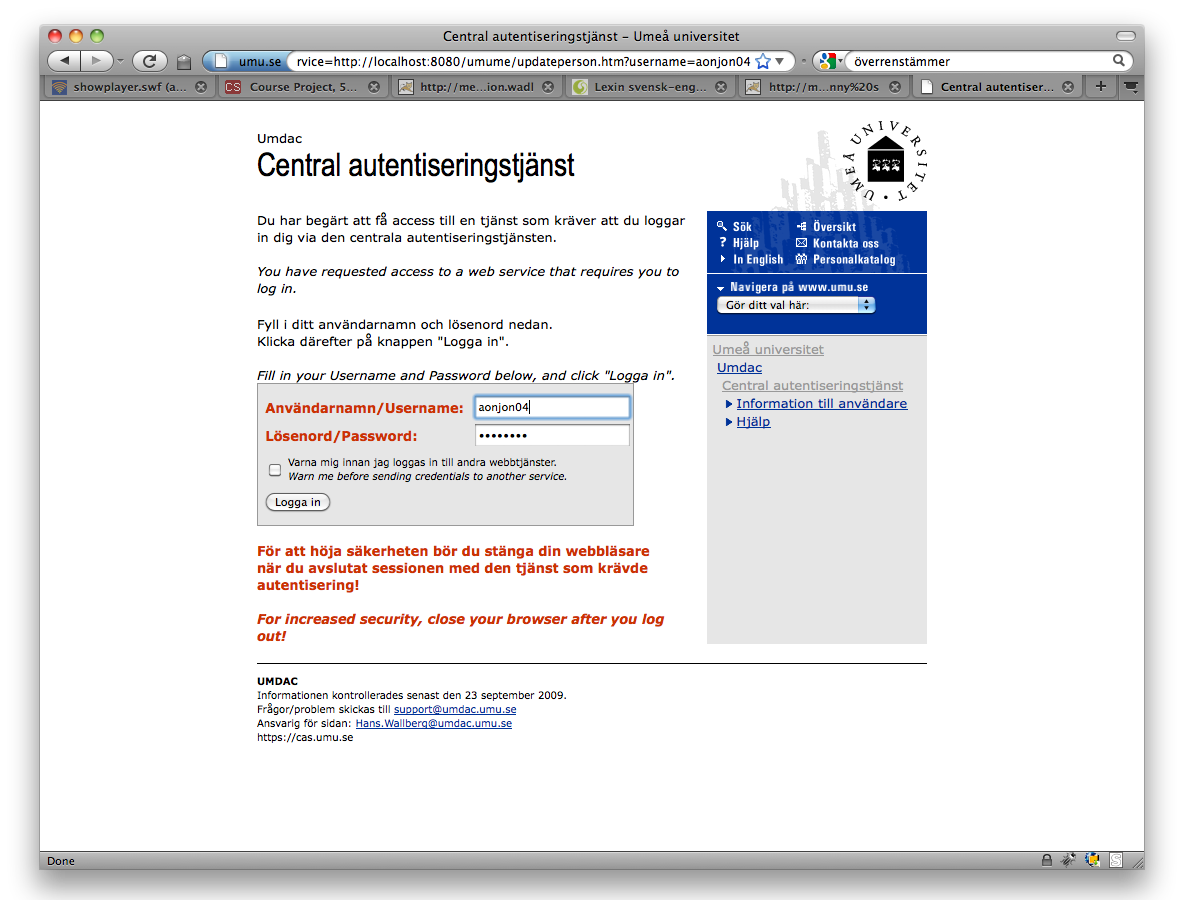
\includegraphics[width=3.3in]{images/pic4.png}
  \caption{Click on "uppdatera" at the bottom of the profile and then authorize CAS-user.}
  \label{fig:images/cas}
\end{figure}

\begin{figure}[!thb]
  \centering
  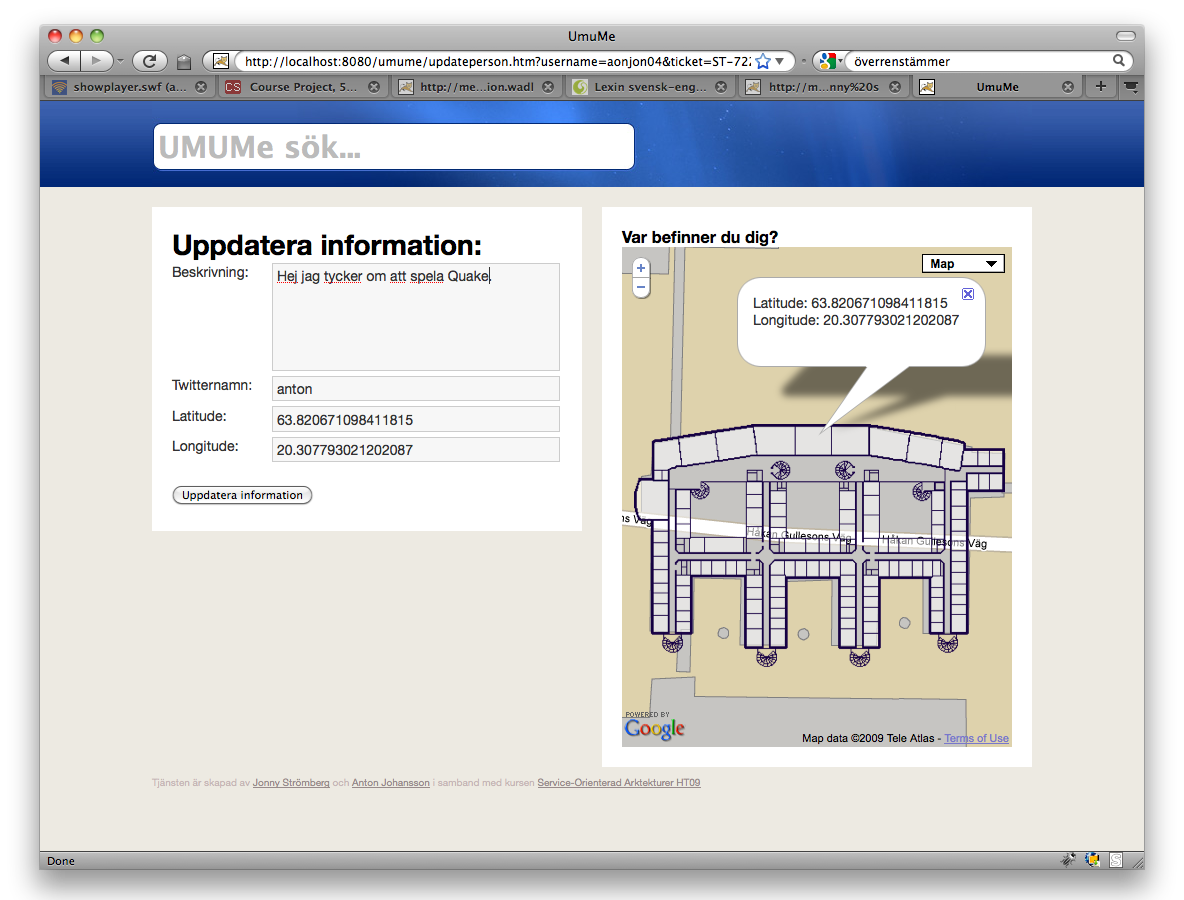
\includegraphics[width=3.3in]{images/pic5.png}
  \caption{Update user information}
  \label{fig:images/edit}
\end{figure}

\begin{figure}[!thb]
  \centering
  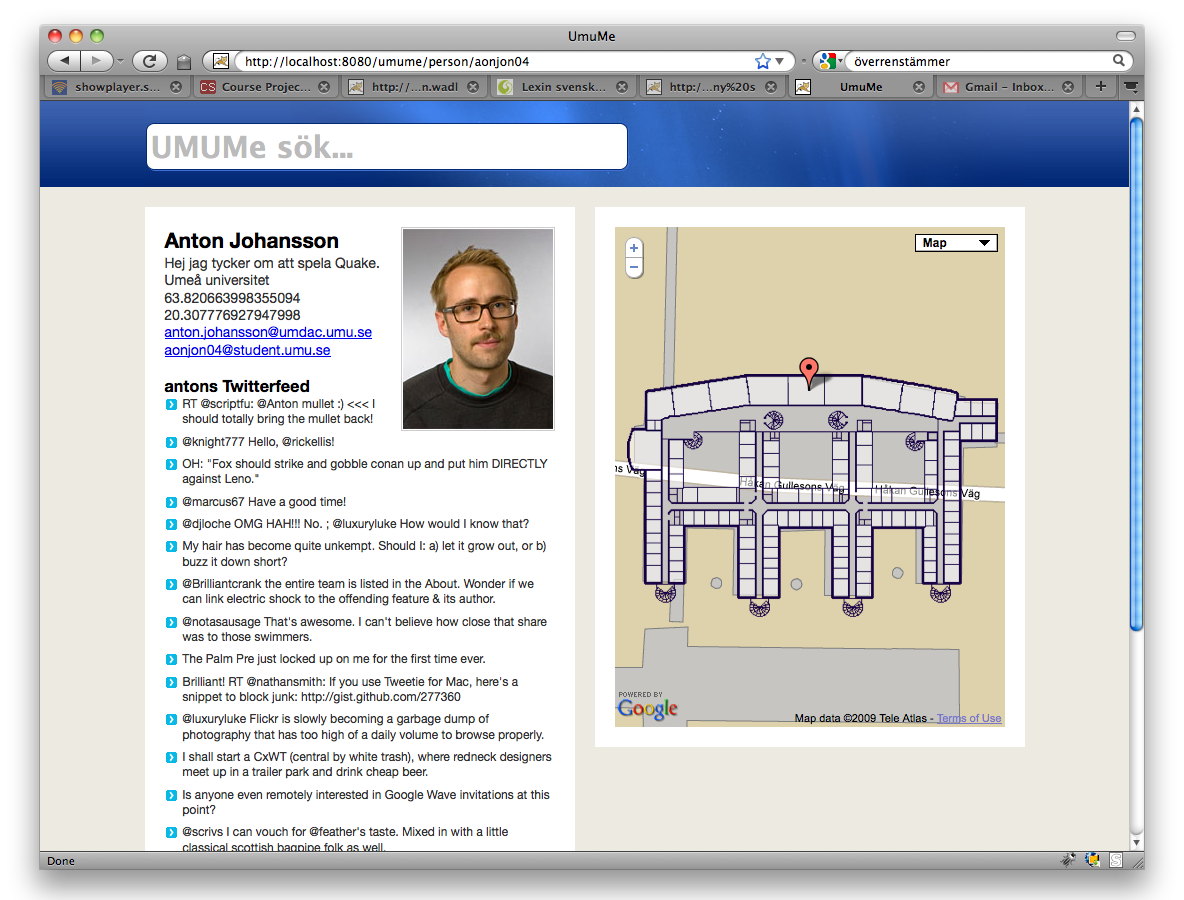
\includegraphics[width=3.3in]{images/pic6.png}
  \caption{See updated information (if the authorized CAS-user was the same as the updated profile.}
  \label{fig:images/edited-user}
\end{figure}

\newpage
\section{System description}\label{sec:system}
% Beskriv översiktligt hur programmet är uppbyggt och hur det löser
% problemet.

% The GCom middleware consists of three (logical) modules, the group
% management module, the communication module and the message ordering
% module. These are, respectively, responsible for handling group
% membership issues, communication message exchange semantics and
% message (re)ordering issues. All of these modules need to function
% properly in order for your system to be able to ensure correct
% message delivery semantics.

\begin{figure*}[!thb]
  \centerline{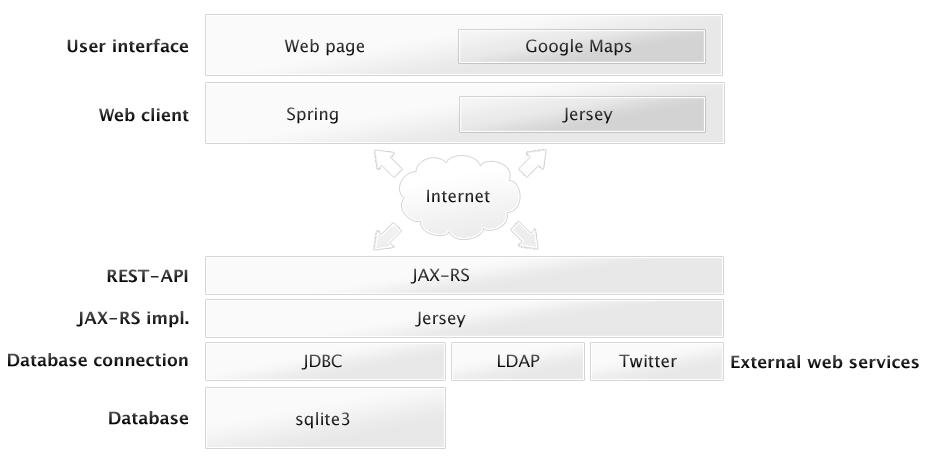
\includegraphics[width=160mm]{images/systemarchitecture.jpg}}
  \caption{GCom stack}
  \label{fig:images/sysarch}
\end{figure*}

The system is consists of different modules, Figure \ref{fig:images/sysarch} gives an overview of the parts.

\subsection{Umume-rest}\label{sec:umume-rest}
The RESTful web service uses the \textit{JAX-RS API}\footnote{\url{http://jcp.org/en/jsr/detail?id=311}} with the \textit{Jersey}\footnote{https://jersey.dev.java.net/} implementation. This enables resources to be defined within normal java classes by merely adding annotations to specify at which path the resource is available and what HTTP-methods the resource is accessable by. Se an example in Code \ref{code:jaxrs}. This is basically what is used by \textit{Umume-rest} to provide resources describing users. A java bean \textit{PersonBean.java} is used to represent users. This bean is marshaled and unmarshaled by JAXB\footnote{\url{https://jaxb.dev.java.net/}} into different mediatypes depending on what is requested. Our user resources can be fetched as XML or JSON\footnote{\url{http://www.json.org/}} depending on which HTTP Accept header is sent by the request.

\begin{code}
  \begin{footnotesize}
\begin{verbatim}
// The resource is available at path /users/{uid}
@Path("/users/{uid}")
public class UsersResource {
    // The Java method will process HTTP GET requests
    @GET
    // It can return XML and JSON
    @Produces({"application/xml",
               "application/json"})
    public Person getUserXML(
                       @PathParam("uid") String uid) {
        //...
        return person;
    }
\end{verbatim}
  \end{footnotesize}
  \caption{JAX-RS resource}\label{code:jaxrs}
\end{code}

\subsubsection{Update user resource}\label{sec:updateuser}
To update a user resource a valid CAS user is required. The request is made by a HTTP PUT request with new information about the referenced user, see example implementation in Code \ref{code:updateResource}. This example consumes XML with updated information about the user resource.

To validate whether the request comes from the same user that requests the change a CAS ticket is required as a query string. This supplied ticket from CAS is validated at \url{https://cas.umu.se} using a CAS-client\footnote{\url{http://www.jasig.org/cas}}. If the supplied ticket is valid a username can be extracted, and if this username is the same as the username of the resource to change it can be certain that the request comes from the person who is represented by the resource. Since a ticket is confidential information all this network traffic is tunneled through a secure connection using the HTTPS protocol. See Figure \ref{fig:images/auth} for an overview of this communication.

\begin{code}
  \begin{footnotesize}
\begin{verbatim}
@PUT
@Consumes(MediaType.APPLICATION_XML)
public Response updateUser(
        @PathParam("uid") String uid,
        PersonBean pb,
        @QueryParam("ticket") String ticket,
        @QueryParam("service") String service) {
        // validate user, persist updated info
        return Response; //200 OK or errorcode
}
\end{verbatim}
  \end{footnotesize}
  \caption{Update resource}\label{code:updateResource}
\end{code}

\begin{figure}[!thb]
  \centering
  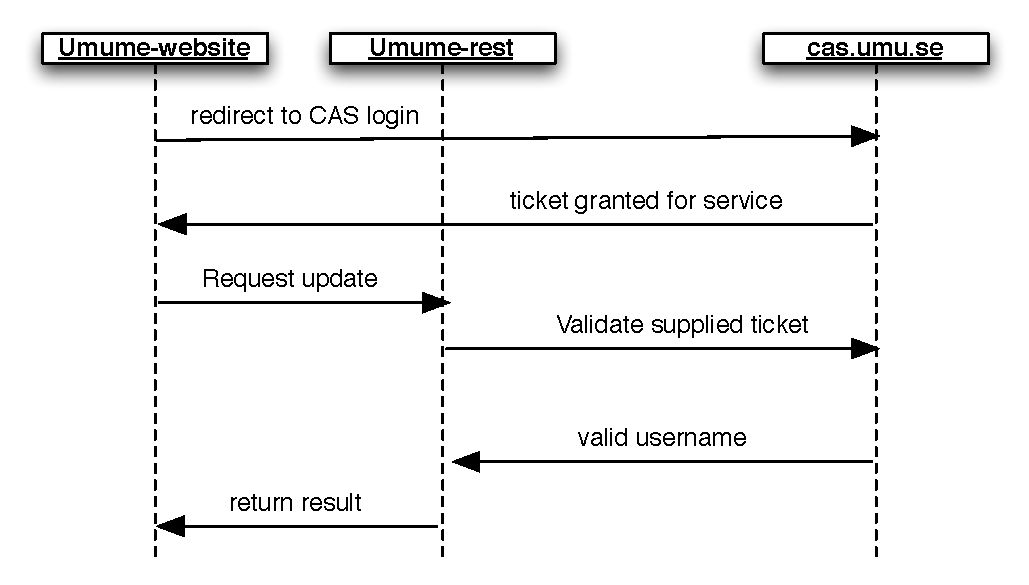
\includegraphics[width=3.3in]{images/auth.pdf}
  \caption{CAS authentication}
  \label{fig:images/auth}
\end{figure}

\subsubsection{Deployment: web.xml}
If \textit{Umume-rest} is compiled and archived into a WAR-file for deployment, the file \texttt{web.xml} need to specify in which package the resources are located, this can be seen in an excerpt from \texttt{web.xml} in Code \ref{code:webxml}. This file also specifies that PUT requests on user resources need to be made with a confidential transporting guarantee.

\begin{code}
  \begin{footnotesize}
\begin{verbatim}
<servlet>
   <servlet-name>UmumeREST</servlet-name>
   <servlet-class>
      com.sun.jersey.spi.container.servlet.ServletContainer
   </servlet-class>
   <init-param>
      <param-name>
         com.sun.jersey.config.property.packages
      </param-name>
      <param-value>
         se.umu.cs.umume.rest.resources
      </param-value>
   </init-param>
</servlet>
\end{verbatim}
  \end{footnotesize}
  \caption{web.xml jersey resources}\label{code:webxml}
\end{code}

\subsubsection{Persistance layer}\label{sec:persistance}

\subsection{Umume-website}\label{sec:umume-website}

The website 

\subsubsection{Spring Framework}\label{springframework}
The web site built with the Spring Framework and uses the MVC 
design pattern. This means that it consist of views (.jsp), models (Java Beans)
and controllers (Java classes). These are defined in a servlet called 
\textit{umume-servlet.xml}.

\subsubsection{Searching}\label{sec:web-search}
The main feature is the search function that is entirely built 
in JavaScript. Searching is done as the user type letters. This
is done with AJAX requests 
\footnote{\url{http://en.wikipedia.org/wiki/Ajax_\%28programming\%29}}
to the Umume-rest web service that serveres data in content-type 
\textit{application/javascript}. 

To make life easier is jQuery \footnote{\url{http://jquery.com/}} used that hels a lot when there is 
AJAX and event-handling involved. See example at \ref{code:jquery}

\begin{code}
  \begin{footnotesize}
\begin{verbatim}
\$.ajax({
       url: "http://mega.cs.umu.se:8080/umume-rest/search/" + searchVal + "?callback=?",
       success: aj.dataLoaded,
       error: aj.failure,
       type: "GET",
       dataType: "json",
       cache: false,
       processData: false
});
\end{verbatim}
  \end{footnotesize}
  \caption{Send request to web service with search string {searchVal}}\label{code:jquery}
\end{code}            



Springframework
Jersey
Sökning JS
Google Maps
URL-filter



\subsubsection{Error handling}\label{sec:error-handling}
% To detect errors: The module monitors a group and indicates when a
% member of the group crashes (or for some other reason become
% unreachable).
When sending messages a group member may detect that one of the
receiving members has crashed. If the detecting member is a group
leader it will directly send a groupchange message, otherwise it will
send a membercrash message which when received by the group leader
will result in a groupchange message multicasted to the group. A
groupchange message contains information about the complete new group
composition whereas a membercrash message only contains information
about the members that have crashed.

When the member that has crashed is the group leader the exact same procedure is used except that when processes receive membercrash messages they will check if they are the new group leader, and if they are they will send a groupchange message to the group. Group members test if they are the new group leader by checking if they have the maximum value of \textit{UUID}s in the current group. This is a variant of the \textit{Bully alghoritm}, see page 482
% TODO: this section maybe should have contained info about normal leave
% messages, which we have not implemented.
% \subsubsection{Group changes}\label{sec:group-changes}
% To notify changes in group membership: The module notifies all group
% members about changes in group composition.


\begin{table}[H]
  \centering
  \begin{footnotesize}
    \begin{tabular} {c | c | c | c}
      % BEGIN RECEIVE ORGTBL casualtotal
      & p1 & p2 & p3 - Sequencer (hold all messages) \\
      \hline
      Send order & one &  &  \\
      & two &  &  \\
      \hline
      &  &  & (Release messages in reverse order) \\
      \hline
      Receive order & one & one & one \\
      & two & two & two \\
      % END RECEIVE ORGTBL casualtotal
    \end{tabular}
  \end{footnotesize}
  \caption{Casual-Total ordering tests}
  \label{tbl:castot}
\end{table}
\begin{comment}
  #+ORGTBL: SEND casualtotal orgtbl-to-latex :splice t
  |               | p1  | p2  | p3 - Sequencer (hold all messages)  |
  |---------------+-----+-----+-------------------------------------|
  | Send order    | one |     |                                     |
  |               | two |     |                                     |
  |---------------+-----+-----+-------------------------------------|
  |               |     |     | (Release messages in reverse order) |
  |---------------+-----+-----+-------------------------------------|
  | Receive order | one | one | one                                 |
  |               | two | two | two                                 |
\end{comment}


\section{Discussion}\label{sec:discussion}
% Vilka problem och begränsningar har din lösning av uppgiften? Hur
% skulle de kunna rättas till?
The following sections will discuss some of the problems and solutions
encountered while implementing \textit{GCom}.

% \section{Reflektioner}\label{Reflektioner}
% % Reflektioner - Var det något som var speciellt krångligt? Vilka
% % problem uppstod och hur löste ni dem? Vilka verktyg använde ni? Hur
% % upplevde ni de verktygen? + Allmänna synpunkter. Om ni har upplevt
% % problem på grund av olika miljöer (i termer av operativsystem och
% % liknande) så kan det även vara intressant att nämna det, samt motivera
% % ert val av miljö.

\subsection{No automatic failure detection}\label{sec:no-automatic-failure-detection}
We have no automatic "ping-function" in our system. That means that if for example
a group member crashed, no one will realize this before they tries to send a message. This also
implies that if the leader crashes and no messages is sent, there will be no way to connect to the group.

\subsection{Security}\label{sec:security}
Here there are great opportunities for development. For instance, theoreticly anyone could send I 
GroupChange-message and noone will know it the sender is the leader or not. It is the same way 
with all other messages types.

\section{Scenarios}\label{sec:scenarios}
This section shows different scenarios that explains how the system
works.


\section{Tests}\label{sec:tests}
% Noggranna testkörningar där man ser att programmet fungerar som det
% ska.

% During your demo, you will need to convince the teachers that your
% implementation works. Bring a test protocol, i.e., a series of tests
% that clearly demonstrates that your GCom fulfills the requirements
% and a test tool which can be used to apply it. The test protocol
% should include, e.g., tests of all message orders and multicast
% types. Bring a copy of the test protocol on paper, see page 491 in
% [DS] for suggested notation. Your test protocol must clearly state
% your names, user names, and which level you intend to demonstrate.

% The fact that a system cannot be formally proven to work does not
% make it impossible to implement - consider for example the Internet.
% Read pages 498 and 508 in [DS].



%%%%%%%%%%%%%%%% END APPENDIX AND STUFF %%%%%%%%%%%%%%%%
%\bibliographystyle{alpha}
%\bibliography{books.bib}

\newpage
\onecolumn
\appendix
\pagenumbering{roman}
\section{Appendix}\label{sec:app}
% % Källkoden ska finnas tillgänglig i er hemkatalog
% % ~/edu/apjava/lab1/. Bifoga även utskriven källkod.
\subsection{Project Specification}\label{app:ps}
\newpage
\subsection{application.wadl}\label{app:wadl}
\begin{code}
  \begin{footnotesize}
\begin{verbatim}
<application>
   <doc jersey:generatedBy="Jersey: 1.0.3 04/16/2009 12:07 AM"/>
   <resources base="http://mega.cs.umu.se:8080/umume-rest/">

      <resource path="/search/{searchString}">
         <param type="xs:string" style="template" name="searchString"/>
         <method name="GET" id="searchForUsers">
            <request>
               <param type="xs:string" style="query" name="callback"/>
            </request>

            <response>
               <representation mediaType="application/javascript"/>
            </response>
         </method>
         <method name="GET" id="searchForUsers">
            <response>
               <representation mediaType="application/xml"/>
               <representation mediaType="application/json"/>
            </response>
         </method>
      </resource>

      <resource path="/users/{uid}">
         <param type="xs:string" style="template" name="uid"/>
         <method name="GET" id="getUserXML">
            <response>
               <representation mediaType="application/xml"/>
               <representation mediaType="application/json"/>
            </response>
         </method>
         <method name="PUT" id="updateUser">
            <request>
               <param type="xs:string" style="query" name="ticket"/>
               <param type="xs:string" style="query" name="service"/>
               <representation mediaType="application/xml"/>
            </request>
            <response>
               <representation mediaType="*/*"/>
            </response>
         </method>
      </resource>

   </resources>
</application>
\end{verbatim}
  \end{footnotesize}
  \caption{WADL}\label{code:wadl}
\end{code}
\end{document}
